
\documentclass[aspectratio=169,11pt]{beamer}

% ---------------------------------------------------------
% APRESENTAÇÃO - COMPUTAÇÃO GRÁFICA / CCO
% Universidade Federal de Ouro Preto - DECOM
% ---------------------------------------------------------

% --- PACOTES ---
\usepackage[utf8]{inputenc}
\usepackage[T1]{fontenc}
\usepackage[brazil]{babel}
\usepackage{amsmath, amssymb}
\usepackage{booktabs}
\usepackage{tabularx}
\usepackage{graphicx}
\usepackage{xcolor}
\usepackage{hyperref}
\usepackage{listings}
\usepackage{tikz}

% --- CORES ---
\definecolor{ufopred}{RGB}{140,29,36}
\definecolor{deepnavy}{RGB}{20,35,60}
\definecolor{lightgray}{RGB}{245,247,250}
\definecolor{darkslate}{RGB}{30,40,50}
\definecolor{softblue}{RGB}{230,238,247}

% --- TEMA ---
\usetheme{Madrid}
\usecolortheme{default}
\setbeamertemplate{navigation symbols}{}
\setbeamercolor{structure}{fg=ufopred}
\setbeamercolor{frametitle}{fg=white,bg=ufopred}
\setbeamercolor{title}{fg=white,bg=ufopred}
\setbeamercolor{block title}{fg=white,bg=deepnavy}
\setbeamercolor{block body}{fg=black,bg=lightgray}
\setbeamercolor{alerted text}{fg=ufopred}

% --- RODAPÉ ---

\setbeamertemplate{footline}{%
  \leavevmode%
  \hbox{%
    \begin{beamercolorbox}[wd=.72\paperwidth,ht=2.6ex,dp=1.1ex,leftskip=1.5ex]{author in head/foot}%
      \textcolor{darkslate}{\insertshorttitle}
    \end{beamercolorbox}%
    \begin{beamercolorbox}[wd=.28\paperwidth,ht=2.6ex,dp=1.1ex,rightskip=1.5ex plus1fil]{date in head/foot}%
      \hfill \textcolor{darkslate}{\insertframenumber/\inserttotalframenumber}
    \end{beamercolorbox}%
  }%
}

% --- CÓDIGO ---
\lstset{
  basicstyle=\ttfamily\small,
  keywordstyle=\color{ufopred}\bfseries,
  commentstyle=\color{darkslate},
  stringstyle=\color{deepnavy},
  showstringspaces=false,
  frame=single,
  rulecolor=\color{lightgray},
  breaklines=true
}

% --- COMANDO PARA FIGURAS ---
\newcommand{\figura}[2][0.8\textwidth]{
\begin{center}
\fcolorbox{deepnavy}{lightgray}{
\begin{minipage}[c][0.28\textheight][c]{#1}
\centering
\textcolor{darkslate}{\textbf{#2}}\\[0.2cm]
\small Inserir captura de tela ou figura.
\end{minipage}}
\end{center}
}

% --- DADOS ---
\title[Visualização CCO -- Computação Gráfica]
{Visualização, Rasterização e Recorte de Árvores Arteriais Geradas por CCO}

\subtitle{Trabalho Prático 1 -- Computação Gráfica}

\author{
Arian Selene Daza Ochoa \and
Bianca Barreto Leme \and
Karina Miyu Kinukawa
}

\institute[UFOP]{
Departamento de Computação (DECOM)\\
Universidade Federal de Ouro Preto
}

\date{2026}

% ---------------------------------------------------------
\begin{document}

% ---------------------------------------------------------
% CAPA
% ---------------------------------------------------------
\begin{frame}
\titlepage
\end{frame}

% ---------------------------------------------------------
% ROTEIRO
% ---------------------------------------------------------

\begin{frame}{Roteiro da Apresentacao}
\tableofcontents
\end{frame}

% =========================================================
\section{Contexto e Objetivos}
% =========================================================

\begin{frame}{Contextualização}
\begin{block}{Contexto}
A Plataforma CCO/UFOP trabalha com a geração de árvores
vasculares sintéticas por meio do método
\textit{Constrained Constructive Optimization} (CCO).
\end{block}

\vspace{0.3cm}

\begin{itemize}
    \item As árvores representam redes de vasos sanguíneos.
    \item Os modelos são disponibilizados em arquivos no formato VTK.
    \item As geometrias podem ser bidimensionais ou tridimensionais.
    \item Cada segmento arterial possui um atributo associado: o raio.
\end{itemize}

\vspace{0.2cm}
\begin{center}
\textbf{Desafio:} desenvolver ferramentas para visualizar,
manipular e explorar essas geometrias.
\end{center}
\end{frame}

% ---------------------------------------------------------
\begin{frame}{Objetivos}
\begin{block}{Objetivo geral}
Desenvolver uma aplicação gráfica para visualização e
manipulação de árvores arteriais geradas pelo método CCO,
aplicando conceitos de Computação Gráfica.
\end{block}

\vspace{0.3cm}

\textbf{Objetivos específicos:}
\begin{itemize}
    \item Carregar e interpretar modelos geométricos em VTK.
    \item Aplicar transformações geométricas em 2D e 3D.
    \item Representar visualmente os atributos dos vasos.
    \item Implementar algoritmos de rasterização.
    \item Implementar e comparar algoritmos de recorte.
\end{itemize}
\end{frame}

% =========================================================
\section{Dados e Metodologia}
% =========================================================

\begin{frame}{Dados Utilizados}
\begin{columns}[T]
\column{0.52\textwidth}

\begin{itemize}
    \item Modelos de árvores arteriais gerados por CCO.
    \item Arquivos no formato \texttt{.vtk}.
    \item Geometrias em duas e três dimensões.
    \item Estrutura composta por pontos e segmentos.
    \item Atributo escalar associado aos segmentos: \texttt{raio}.
\end{itemize}

\column{0.44\textwidth}

\begin{block}{Exemplo de modelo analisado}
\small
\begin{tabular}{ll}
\toprule
Característica & Valor \\
\midrule
Pontos & 128 \\
Segmentos & 127 \\
Raio mínimo & 0,2052 \\
Raio máximo & 1,0178 \\
Dimensão & 3D \\
\bottomrule
\end{tabular}
\end{block}

\end{columns}
\end{frame}

% ---------------------------------------------------------
\begin{frame}{Representação dos Dados}
\begin{block}{Modelo geométrico}
A árvore arterial é representada como um grafo:
\[
G=(V,E)
\]
\end{block}

\begin{itemize}
    \item $V$: conjunto de pontos que representam bifurcações
    e extremidades dos vasos.
    \item $E$: conjunto de segmentos que conectam os pontos.
    \item Cada segmento possui um raio associado.
\end{itemize}

\vspace{0.3cm}

\begin{columns}[c]
    \begin{column}{0.48\textwidth}
        \centering
        \textbf{Representação 2D}
        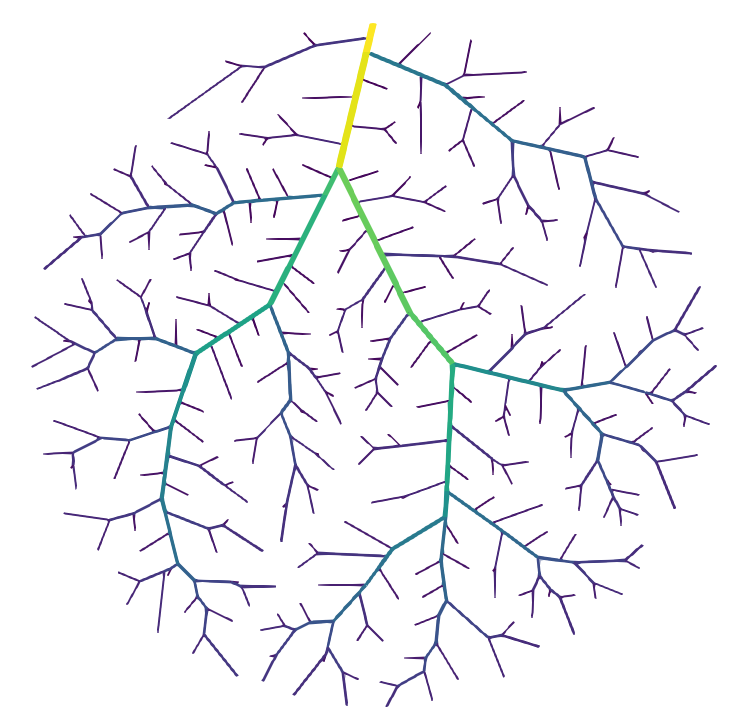
\includegraphics[width=\textwidth,height=0.35\textheight,keepaspectratio]{img/tree2d.png}
    \end{column}

    \begin{column}{0.48\textwidth}
        \centering
        \textbf{Representação 3D}
        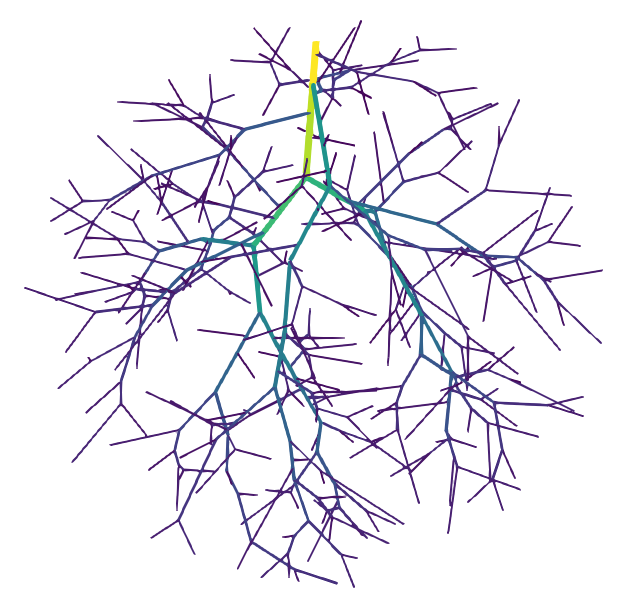
\includegraphics[width=\textwidth,height=0.35\textheight,keepaspectratio]{img/tree3d.png}
    \end{column}
\end{columns}
\end{frame}

% ---------------------------------------------------------
\begin{frame}{Tecnologias e Arquitetura}
\begin{columns}[T]
\column{0.48\textwidth}

\textbf{Tecnologias}
\begin{itemize}
    \item Python.
    \item PyVista e VTK.
    \item PySide6 para interface gráfica.
    \item NumPy para operações numéricas.
\end{itemize}

\column{0.48\textwidth}

\textbf{Organização modular}
\begin{itemize}
    \item \texttt{core/}: carregamento dos modelos.
    \item \texttt{rasterization/}: rasterização.
    \item \texttt{clipping/}: algoritmos de recorte.
    \item \texttt{visualization/}: transformações e visualização.
    \item \texttt{interface/}: interface gráfica.
\end{itemize}

\end{columns}

\vspace{0.3cm}

\begin{center}
A separação em módulos permite desenvolver e testar
as técnicas de forma independente.
\end{center}
\end{frame}

% ---------------------------------------------------------
\begin{frame}{Fluxo Geral da Aplicação}
\begin{center}
\begin{tikzpicture}[
    node distance=0.65cm,
    every node/.style={
        draw,
        rounded corners,
        align=center,
        minimum width=5.2cm,
        minimum height=0.65cm,
        fill=lightgray
    }
]
\node (vtk) {Leitura dos arquivos VTK};
\node (geom) [below of=vtk] {Extração da geometria e dos atributos};
\node (trans) [below of=geom] {Transformações geométricas e visualização};
\node (alg) [below of=trans] {Aplicação dos algoritmos gráficos};
\node (out) [below of=alg, fill=softblue] {Resultados visuais e interativos};

\draw[->, thick, ufopred] (vtk) -- (geom);
\draw[->, thick, ufopred] (geom) -- (trans);
\draw[->, thick, ufopred] (trans) -- (alg);
\draw[->, thick, ufopred] (alg) -- (out);
\end{tikzpicture}
\end{center}
\end{frame}

% =========================================================
\section{Implementação}
% =========================================================
\begin{frame}{Visualização e Atributos}
\begin{columns}[T]
    \column{0.48\textwidth}

    \begin{itemize}
        \item Representação dos vasos por segmentos e tubos.
        \item Visualização de modelos 2D e 3D.
        \item Utilização do atributo \texttt{raio}.
        \item Mapeamento de valores para cores.
    \end{itemize}

    \column{0.48\textwidth}
    \centering
    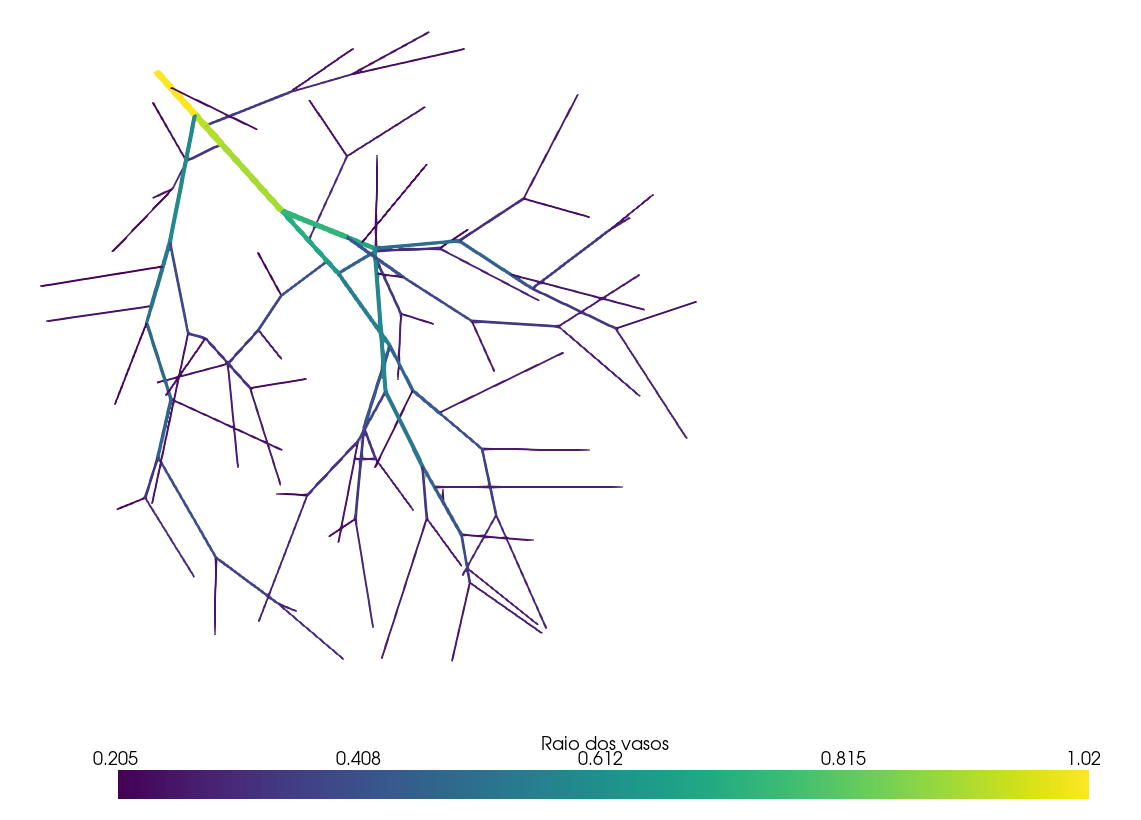
\includegraphics[width=\textwidth,height=0.65\textheight,keepaspectratio]
    {img/tree3d-barra.png}
\end{columns}

\vspace{0.2cm}

\begin{center}
    O mapa de cores permite distinguir visualmente
    segmentos com diferentes raios.
\end{center}
\end{frame}

% ---------------------------------------------------------
\begin{frame}{Transformações Geométricas}
As transformações permitem modificar a posição,
a orientação e as dimensões dos modelos.

\vspace{0.3cm}

\begin{columns}[T]
\column{0.32\textwidth}
\begin{block}{Translação}
Deslocamento da geometria nos eixos.
\end{block}

\column{0.32\textwidth}
\begin{block}{Rotação}
Alteração da orientação do modelo.
\end{block}

\column{0.32\textwidth}
\begin{block}{Escala}
Ampliação ou redução da geometria.
\end{block}
\end{columns}

\vspace{0.4cm}

\begin{center}
As transformações são representadas por matrizes
em coordenadas homogêneas.
\end{center}
\end{frame}

% ---------------------------------------------------------

\begin{frame}{Rasterização de Linhas: Bresenham}
\begin{block}{Objetivo}
Converter segmentos geométricos contínuos em uma sequência
de pixels em uma grade discreta.
\end{block}

\vspace{0.2cm}

\begin{columns}[T]
    \begin{column}{0.52\textwidth}
        \begin{itemize}
            \item Utiliza uma variável de decisão para escolher
            o próximo pixel.
            \item Emprega operações aritméticas inteiras.
            \item Evita o cálculo de coordenadas fracionárias
            a cada passo.
        \end{itemize}

        \vspace{0.2cm}
        A decisão inicial, para o caso de inclinação entre 0 e 1, é:
        \[
        D_0 = 2\Delta y - \Delta x
        \]
    \end{column}

    \begin{column}{0.45\textwidth}
        \centering
        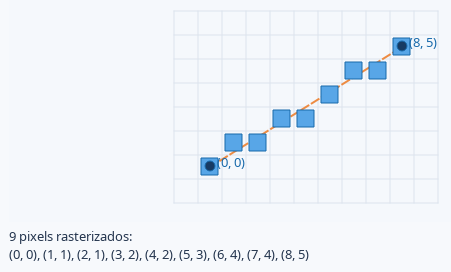
\includegraphics[width=\textwidth,height=0.55\textheight,
        keepaspectratio]{img/bresenham.png}
        
        {\scriptsize Exemplo de rasterização pelo algoritmo de Bresenham.}
    \end{column}
\end{columns}
\end{frame}


% ---------------------------------------------------------

\begin{frame}{Preenchimento de Polígonos: Scanline}

\begin{block}{Objetivo}
Determinar os pixels internos de um polígono por meio
de linhas horizontais de varredura.
\end{block}

\vspace{0.2cm}

\begin{columns}[T]
    \column{0.48\textwidth}
    \centering
    \textbf{Representação geométrica}

    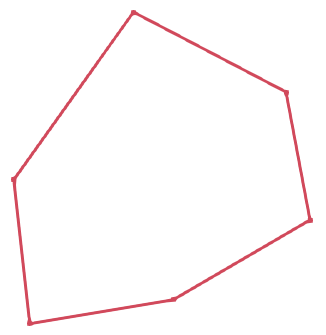
\includegraphics[width=\textwidth,
    height=0.40\textheight,keepaspectratio]
    {img/scanline-pol.png}

    \column{0.48\textwidth}
    \centering
    \textbf{Tabela de Arestas}

    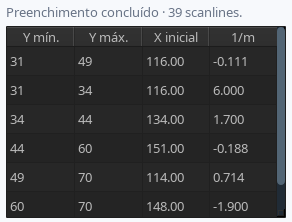
\includegraphics[width=\textwidth,
    height=0.40\textheight,keepaspectratio]
    {img/scanline-table.png}
\end{columns}

\vspace{0.2cm}

\begin{itemize}
    \item Armazenamento dos limites verticais de cada aresta.
    \item Cálculo da interseção inicial e da variação horizontal.
    \item Atualização das interseções durante a varredura.
\end{itemize}

\end{frame}

% ---------------------------------------------------------
\begin{frame}{Recorte de Segmentos: Cohen-Sutherland}
\begin{block}{Objetivo}
Determinar a parte de um segmento de reta que permanece
dentro de uma janela retangular.
\end{block}

\vspace{0.2cm}

\begin{itemize}
    \item Cada extremidade recebe um código de região de 4 bits.
    \item Os códigos indicam a posição em relação à janela.
    \item O algoritmo utiliza operações lógicas para decidir
    se o segmento pode ser aceito ou rejeitado.
\end{itemize}

\vspace{0.2cm}

\begin{block}{Casos triviais}
\begin{itemize}
    \item Aceitação: ambos os códigos são $0000$.
    \item Rejeição: operação AND entre os códigos diferente de zero.
    \item Caso contrário: é necessário calcular intersecções.
\end{itemize}
\end{block}
\end{frame}

% ---------------------------------------------------------
\begin{frame}{Recorte de Segmentos: Liang-Barsky}
\begin{block}{Ideia principal}
Representar o segmento por uma equação paramétrica
e determinar o intervalo de parâmetros que permanece
dentro da janela.
\end{block}

\[
P(t)=P_1+t(P_2-P_1), \quad 0\leq t\leq 1
\]

\vspace{0.2cm}

\begin{itemize}
    \item Analisa as restrições impostas pelas quatro bordas.
    \item Atualiza os limites inferior e superior do parâmetro $t$.
    \item Calcula somente as intersecções necessárias.
\end{itemize}

\vspace{0.2cm}

\begin{center}
\textbf{Comparação:} Cohen-Sutherland utiliza códigos de região,
enquanto Liang-Barsky utiliza intervalos paramétricos.
\end{center}
\end{frame}

% ---------------------------------------------------------
\begin{frame}{Recorte de Polígonos: Sutherland-Hodgman}

\begin{block}{Objetivo}
Recortar um polígono contra uma janela retangular,
produzindo uma nova lista de vértices.
\end{block}

\vspace{0.15cm}

\begin{columns}[T]

    \column{0.53\textwidth}

    O algoritmo percorre o polígono,
    considerando cada borda da janela de recorte.

    \vspace{0.15cm}

    \begin{itemize}
        \item Interno $\rightarrow$ interno: mantém o vértice.
        \item Interno $\rightarrow$ externo: adiciona a intersecção.
        \item Externo $\rightarrow$ interno: adiciona intersecção e vértice.
        \item Externo $\rightarrow$ externo: descarta ambos.
    \end{itemize}

    \column{0.43\textwidth}

    \centering
    \textbf{Resultado do recorte}

    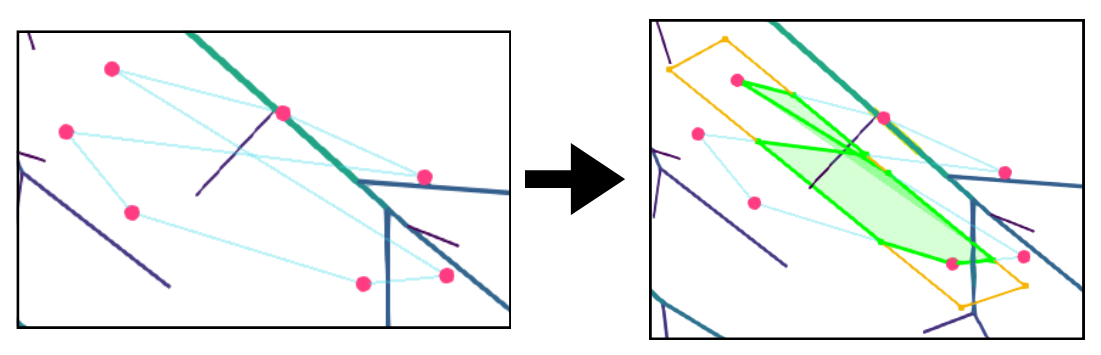
\includegraphics[width=\textwidth,
    height=0.43\textheight,keepaspectratio]
    {img/sh.png}

\end{columns}

\vspace{0.1cm}

\begin{center}
    {\scriptsize O polígono resultante contém apenas a região
    interna à janela de recorte.}
\end{center}

\end{frame}

% =========================================================
\section{Resultados}
% =========================================================

\begin{frame}{Resultados da Aplicação}

\begin{columns}[T]

    \column{0.48\textwidth}
    \centering
    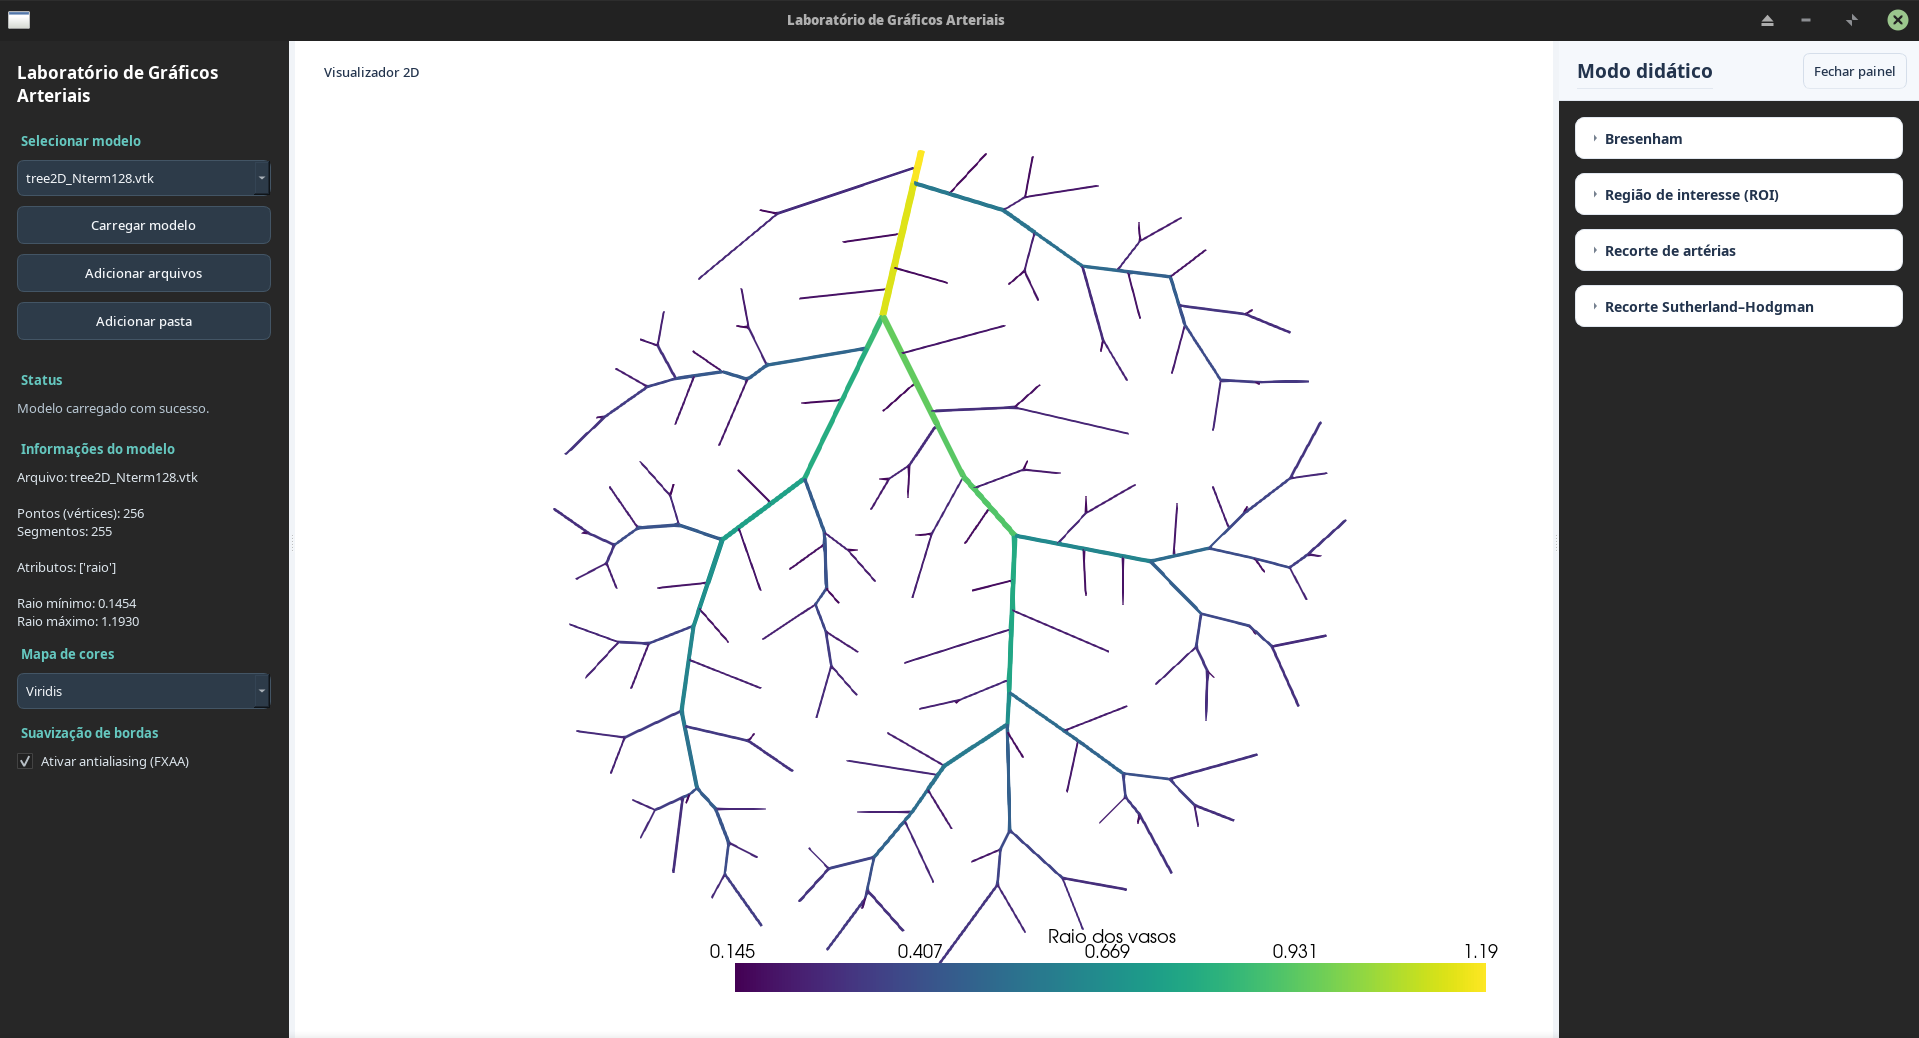
\includegraphics[width=0.95\textwidth,
    height=0.38\textheight,keepaspectratio]
    {img/inter2d.png}

    {\scriptsize Interface e ferramentas disponíveis.}

    \column{0.48\textwidth}
    \centering
    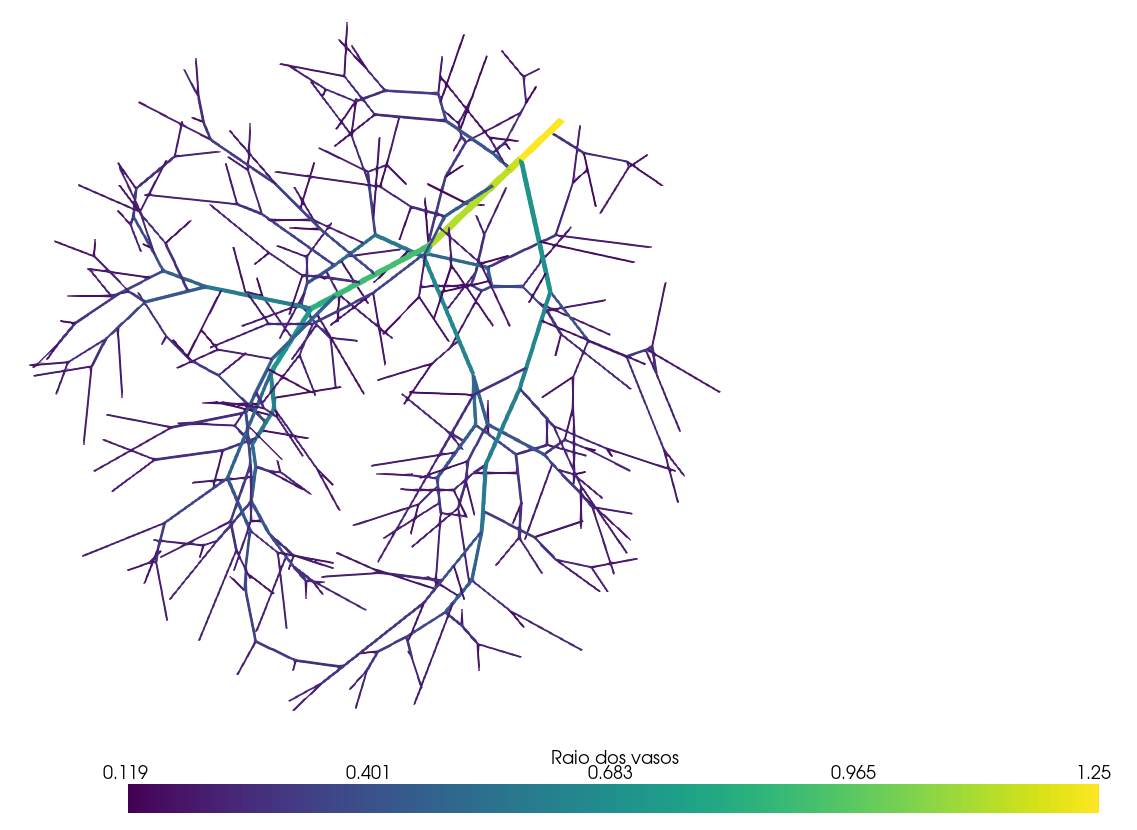
\includegraphics[width=0.95\textwidth,
    height=0.38\textheight,keepaspectratio]
    {img/tree3d-raio.png}

    {\scriptsize Modelo vascular com representação dos raios.}

\end{columns}

\vspace{0.25cm}

\begin{itemize}
    \item Carregamento e visualização de modelos vasculares 2D e 3D.
    \item Aplicação de técnicas de rasterização e recorte.
    \item Exploração interativa das geometrias.
\end{itemize}

\end{frame}

% ---------------------------------------------------------
\begin{frame}{Comparação dos Algoritmos de Recorte}
\small

Resultados apresentados para uma árvore com
$N_{\text{term}}=256$, contendo 511 segmentos.

\vspace{0.2cm}

\begin{center}
\begin{tabular}{lcc}
\toprule
\textbf{Algoritmo} & \textbf{Cenário} & \textbf{Tempo médio (ms)} \\
\midrule
Cohen-Sutherland & Aceite/rejeição trivial & 1,12 \\
Cohen-Sutherland & Recorte frequente & 3,85 \\
Liang-Barsky & Recorte frequente & 2,68 \\
Sutherland-Hodgman & Recorte poligonal & 4,20 \\
\bottomrule
\end{tabular}
\end{center}

\vspace{0.3cm}

\begin{block}{Observação}
Nos cenários de recorte frequente, Liang-Barsky apresentou
tempo aproximadamente 30\% menor que Cohen-Sutherland.
\end{block}
\end{frame}

% ---------------------------------------------------------
\begin{frame}{Discussão dos Resultados}
\begin{itemize}
    \item Bresenham preservou a continuidade dos segmentos
    na rasterização em 8-vizinhança.
    
    \vspace{0.15cm}
    \item Cohen-Sutherland apresentou bom desempenho
    em situações de aceitação e rejeição triviais.
    
    \vspace{0.15cm}
    \item Liang-Barsky apresentou vantagem nos cenários
    com intersecções frequentes.
    
    \vspace{0.15cm}
    \item A organização modular facilita a extensão
    e a manutenção da aplicação.
\end{itemize}
\end{frame}

% =========================================================
\section{Conclusão}
% =========================================================

\begin{frame}{Conclusões}
\begin{itemize}
    \item Foi desenvolvida uma aplicação para visualização
    e manipulação de árvores arteriais CCO.
    
    \vspace{0.2cm}
    \item Foram implementadas técnicas de transformação,
    rasterização e recorte geométrico.
    
    \vspace{0.2cm}
    \item Os algoritmos possibilitaram explorar diferentes
    estratégias de processamento gráfico.
    
    \vspace{0.2cm}
    \item A aplicação constitui uma base modular para
    experimentação e visualização científica.
\end{itemize}

\vspace{0.3cm}

\begin{block}{Trabalhos futuros}
Investigar técnicas adicionais de antialiasing e estender
os algoritmos de recorte para volumes tridimensionais.
\end{block}
\end{frame}

% ---------------------------------------------------------
\begin{frame}{Referências}
\footnotesize

\begin{thebibliography}{99}

\bibitem{bresenham}
BRESENHAM, J. E.
Algorithm for computer control of a digital plotter.
\textit{IBM Systems Journal}, v. 4, n. 1, p. 25--30, 1965.

\bibitem{foley}
FOLEY, J. D. et al.
\textit{Computer Graphics: Principles and Practice}.
3. ed. Boston: Addison-Wesley Professional, 2013.

\bibitem{liang}
LIANG, Y. D.; BARSKY, B. A.
A new concept and algorithm for line clipping.
\textit{ACM Transactions on Graphics}, v. 3, n. 1, p. 1--22, 1984.

\bibitem{schreiner}
SCHREINER, W.; BUXBAUM, P.
Computer-optimization of vascular trees.
\textit{IEEE Transactions on Biomedical Engineering},
v. 40, n. 5, p. 482--491, 1993.

\bibitem{sutherland}
SUTHERLAND, I. E.; HODGMAN, G. W.
Reentrant polygon clipping.
\textit{Communications of the ACM}, v. 17, n. 1, p. 32--42, 1974.

\end{thebibliography}
\end{frame}

% ---------------------------------------------------------
\begin{frame}{Agradecimentos}
\begin{center}
{\Huge\textcolor{ufopred}{Obrigada!}}

\vspace{0.5cm}

{\Large Perguntas?}

\vspace{0.7cm}

Departamento de Computação -- DECOM\\
Universidade Federal de Ouro Preto -- UFOP
\end{center}
\end{frame}

\end{document}
